\begin{figure}[htbp]
	\centering
	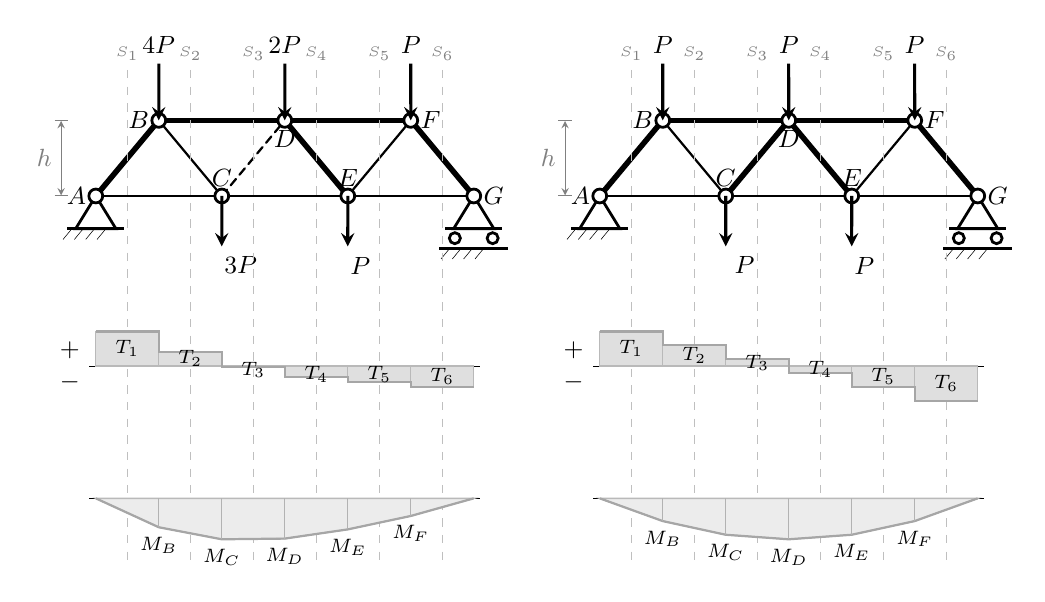
\begin{tikzpicture}[
		scale=0.80,
		comp/.style={line width=2.0pt, line cap=round, line join=round, black},
		tens/.style={line width=0.8pt, line cap=round, line join=round, black},
		zero/.style={line width=0.8pt, line cap=round, line join=round, black,
			dash pattern=on 3pt off 2pt},
		nodo/.style={circle, fill=white, draw=black,
			inner sep=0pt, minimum size=5pt, line width=1.0pt},
		forza/.style={->, >=stealth, line width=1.1pt},
		sez/.style={very thin, gray!50, dashed},
		Tfill/.style={fill=gray!25, draw=gray!55, line width=0.5pt},
		Mfill/.style={fill=gray!15, draw=gray!55, line width=0.5pt},
		Mtick/.style={gray!60, line width=0.5pt},
		]
		
		%%-- COLONNA 1 -------------------------------------------------------
		\coordinate (A)  at (0,0);
		\coordinate (C1) at (2,0);
		\coordinate (E1) at (4,0);
		\coordinate (G)  at (6,0);
		\coordinate (B1) at (1,1.2);
		\coordinate (D1) at (3,1.2);
		\coordinate (F1) at (5,1.2);
		
		%% corrente inferiore: teso (sottile)
		\draw[tens](A)--(C1)--(E1)--(G);
		%% corrente superiore: compresso (spesso)
		\draw[comp](B1)--(D1)--(F1);
		%% diagonali col 1:
		%% AB: salente, T1>0 → compressa
		\draw[comp](A)--(B1);
		%% BC: discendente, T2>0 → tesa
		\draw[tens](B1)--(C1);
		%% CD: salente, T3≈0 → scarica
		\draw[zero](C1)--(D1);
		%% DE: discendente, T4<0 → compressa
		\draw[comp](D1)--(E1);
		%% EF: salente, T5<0 → tesa
		\draw[tens](E1)--(F1);
		%% FG: discendente, T6<0 → compressa
		\draw[comp](F1)--(G);
		
		\foreach \pt in {C1,E1,B1,D1,F1}{\node[nodo]at(\pt){};}
		
		\node[left,  font=\small]at(A)  {$A$};
		\node[left,  font=\small]at(B1) {$B$};
		\node[above, font=\small]at(C1) {$C$};
		\node[below, font=\small]at(D1) {$D$};
		\node[above, font=\small]at(E1) {$E$};
		\node[right, font=\small]at(F1) {$F$};
		\node[right, font=\small]at(G)  {$G$};
		
		\draw[ |<->|,>=stealth,very thin,gray]
		(-0.55,0)--(-0.55,1.2)node[midway,left,font=\small]{$h$};
		
		\draw[forza](1,2.1)--(B1);  \node[above,font=\small]at(1,2.1){$4P$};
		\draw[forza](C1)--(2,-0.8); \node[below,font=\small]at(2.3,-0.8){$3P$};
		\draw[forza](3,2.1)--(D1);  \node[above,font=\small]at(3,2.1){$2P$};
		\draw[forza](E1)--(4,-0.8); \node[above,font=\small]at(4.2,-1.4){$P$};
		\draw[forza](5,2.1)--(F1);  \node[above,font=\small]at(5,2.1){$P$};
		
		\draw[line width=1.0pt](A)--++(-0.32,-0.52)--++(0.64,0)--cycle;
		\draw[line width=1.0pt](-0.45,-0.52)--(0.45,-0.52);
		\foreach \xx in {-0.38,-0.20,-0.02,0.16}
		\draw[very thin](\xx,-0.52)--++(-0.14,-0.17);
		\node[nodo]at(A){};
		
		\draw[line width=1.0pt](G)--++(-0.32,-0.52)--++(0.64,0)--cycle;
		\draw[line width=1.0pt](5.55,-0.52)--(6.45,-0.52);
		\draw[line width=1.0pt](5.70,-0.67)circle(2.5pt);
		\draw[line width=1.0pt](6.30,-0.67)circle(2.5pt);
		\draw[line width=1.0pt](5.45,-0.83)--(6.55,-0.83);
		\foreach \xx in {-0.38,-0.20,-0.02,0.16}
		\draw[very thin](6+\xx,-0.83)--++(-0.14,-0.17);
		\node[nodo]at(G){};
		
		\foreach \xs/\lab in {0.5/$S_1$,1.5/$S_2$,2.5/$S_3$,3.5/$S_4$,4.5/$S_5$,5.5/$S_6$}{
			\draw[sez](\xs,2.0)--(\xs,-5.80);
			\node[above,font=\tiny,gray]at(\xs,2.0){\lab};}
		
		%% taglio col 1
		\draw[thin](-0.1,-2.7)--(6.1,-2.7);
		\node[left,font=\small]at(-0.1,-2.45){$+$};
		\node[left,font=\small]at(-0.1,-2.95){$-$};
		\fill[Tfill](0,-2.7)rectangle(1,-2.15);
		\fill[Tfill](1,-2.7)rectangle(2,-2.472);
		\fill[Tfill](2,-2.713)rectangle(3,-2.7);
		\fill[Tfill](3,-2.875)rectangle(4,-2.7);
		\fill[Tfill](4,-2.955)rectangle(5,-2.7);
		\fill[Tfill](5,-3.036)rectangle(6,-2.7);
		\draw[gray!70,line width=0.8pt]
		(0,-2.15)--(1,-2.15)--(1,-2.472)--(2,-2.472)--
		(2,-2.713)--(3,-2.713)--(3,-2.875)--(4,-2.875)--
		(4,-2.955)--(5,-2.955)--(5,-3.036)--(6,-3.036);
		\node[font=\scriptsize]at(0.5,-2.42){$T_1$};
		\node[font=\scriptsize]at(1.5,-2.58){$T_2$};
		\node[font=\scriptsize]at(2.5,-2.76){$T_3$};
		\node[font=\scriptsize]at(3.5,-2.83){$T_4$};
		\node[font=\scriptsize]at(4.5,-2.83){$T_5$};
		\node[font=\scriptsize]at(5.5,-2.87){$T_6$};
		
		%% momento col 1
		\draw[thin](-0.1,-4.8)--(6.1,-4.8);
		\fill[Mfill]
		(0,-4.8)--(1,-5.259)--(2,-5.450)--(3,-5.439)--
		(4,-5.293)--(5,-5.080)--(6,-4.8)--cycle;
		\draw[gray!70,line width=0.8pt]
		(0,-4.8)--(1,-5.259)--(2,-5.450)--(3,-5.439)--
		(4,-5.293)--(5,-5.080)--(6,-4.8);
		\draw[Mtick](1,-4.8)--(1,-5.259); \node[font=\scriptsize,below]at(1,-5.259){$M_B$};
		\draw[Mtick](2,-4.8)--(2,-5.450); \node[font=\scriptsize,below]at(2,-5.450){$M_C$};
		\draw[Mtick](3,-4.8)--(3,-5.439); \node[font=\scriptsize,below]at(3,-5.439){$M_D$};
		\draw[Mtick](4,-4.8)--(4,-5.293); \node[font=\scriptsize,below]at(4,-5.293){$M_E$};
		\draw[Mtick](5,-4.8)--(5,-5.080); \node[font=\scriptsize,below]at(5,-5.080){$M_F$};
		
		%%-- COLONNA 2 -------------------------------------------------------
		\coordinate (A2) at (8,0);
		\coordinate (C2) at (10,0);
		\coordinate (E2) at (12,0);
		\coordinate (G2) at (14,0);
		\coordinate (B2) at (9,1.2);
		\coordinate (D2) at (11,1.2);
		\coordinate (F2) at (13,1.2);
		
		%% corrente inferiore: teso
		\draw[tens](A2)--(C2)--(E2)--(G2);
		%% corrente superiore: compresso
		\draw[comp](B2)--(D2)--(F2);
		%% diagonali col 2:
		%% AB: salente, T1>0 → compressa
		\draw[comp](A2)--(B2);
		%% BC: discendente, T2>0 → tesa
		\draw[tens](B2)--(C2);
		%% CD: salente, T3>0 → compressa
		\draw[comp](C2)--(D2);
		%% DE: discendente, T4<0 → compressa
		\draw[comp](D2)--(E2);
		%% EF: salente, T5<0 → tesa
		\draw[tens](E2)--(F2);
		%% FG: discendente, T6<0 → compressa
		\draw[comp](F2)--(G2);
		
		\foreach \pt in {C2,E2,B2,D2,F2}{\node[nodo]at(\pt){};}
		
		\node[left, font=\small]at(A2){$A$};
		\node[left, font=\small]at(B2){$B$};
		\node[above,font=\small]at(C2){$C$};
		\node[below,font=\small]at(D2){$D$};
		\node[above,font=\small]at(E2){$E$};
		\node[right,font=\small]at(F2){$F$};
		\node[right,font=\small]at(G2){$G$};
		
		\draw[ |<->|,>=stealth,very thin,gray]
		(7.45,0)--(7.45,1.2)node[midway,left,font=\small]{$h$};
		
		\draw[forza](9,2.1)--(B2);   \node[above,font=\small]at(9,2.1){$P$};
		\draw[forza](C2)--(10,-0.8); \node[below,font=\small]at(10.3,-0.8){$P$};
		\draw[forza](11,2.1)--(D2);  \node[above,font=\small]at(11,2.1){$P$};
		\draw[forza](E2)--(12,-0.8); \node[above,font=\small]at(12.2,-1.4){$P$};
		\draw[forza](13,2.1)--(F2);  \node[above,font=\small]at(13,2.1){$P$};
		
		\draw[line width=1.0pt](A2)--++(-0.32,-0.52)--++(0.64,0)--cycle;
		\draw[line width=1.0pt](7.55,-0.52)--(8.45,-0.52);
		\foreach \xx in {-0.38,-0.20,-0.02,0.16}
		\draw[very thin](8+\xx,-0.52)--++(-0.14,-0.17);
		\node[nodo]at(A2){};
		
		\draw[line width=1.0pt](G2)--++(-0.32,-0.52)--++(0.64,0)--cycle;
		\draw[line width=1.0pt](13.55,-0.52)--(14.45,-0.52);
		\draw[line width=1.0pt](13.70,-0.67)circle(2.5pt);
		\draw[line width=1.0pt](14.30,-0.67)circle(2.5pt);
		\draw[line width=1.0pt](13.45,-0.83)--(14.55,-0.83);
		\foreach \xx in {-0.38,-0.20,-0.02,0.16}
		\draw[very thin](14+\xx,-0.83)--++(-0.14,-0.17);
		\node[nodo]at(G2){};
		
		\foreach \xs/\lab in {8.5/$S_1$,9.5/$S_2$,10.5/$S_3$,11.5/$S_4$,12.5/$S_5$,13.5/$S_6$}{
			\draw[sez](\xs,2.0)--(\xs,-5.80);
			\node[above,font=\tiny,gray]at(\xs,2.0){\lab};}
		
		%% taglio col 2
		\draw[thin](7.9,-2.7)--(14.1,-2.7);
		\node[left,font=\small]at(7.9,-2.45){$+$};
		\node[left,font=\small]at(7.9,-2.95){$-$};
		\fill[Tfill]( 8,-2.7)rectangle( 9,-2.15);
		\fill[Tfill]( 9,-2.7)rectangle(10,-2.37);
		\fill[Tfill](10,-2.7)rectangle(11,-2.59);
		\fill[Tfill](11,-2.81)rectangle(12,-2.7);
		\fill[Tfill](12,-3.03)rectangle(13,-2.7);
		\fill[Tfill](13,-3.25)rectangle(14,-2.7);
		\draw[gray!70,line width=0.8pt]
		(8,-2.15)--(9,-2.15)--(9,-2.37)--(10,-2.37)--
		(10,-2.59)--(11,-2.59)--(11,-2.81)--(12,-2.81)--
		(12,-3.03)--(13,-3.03)--(13,-3.25)--(14,-3.25);
		\node[font=\scriptsize]at( 8.5,-2.42){$T_1$};
		\node[font=\scriptsize]at( 9.5,-2.53){$T_2$};
		\node[font=\scriptsize]at(10.5,-2.65){$T_3$};
		\node[font=\scriptsize]at(11.5,-2.75){$T_4$};
		\node[font=\scriptsize]at(12.5,-2.87){$T_5$};
		\node[font=\scriptsize]at(13.5,-2.98){$T_6$};
		
		%% momento col 2
		\draw[thin](7.9,-4.8)--(14.1,-4.8);
		\fill[Mfill]
		(8,-4.8)--(9,-5.161)--(10,-5.378)--(11,-5.450)--
		(12,-5.378)--(13,-5.161)--(14,-4.8)--cycle;
		\draw[gray!70,line width=0.8pt]
		(8,-4.8)--(9,-5.161)--(10,-5.378)--(11,-5.450)--
		(12,-5.378)--(13,-5.161)--(14,-4.8);
		\draw[Mtick]( 9,-4.8)--( 9,-5.161); \node[font=\scriptsize,below]at( 9,-5.161){$M_B$};
		\draw[Mtick](10,-4.8)--(10,-5.378); \node[font=\scriptsize,below]at(10,-5.378){$M_C$};
		\draw[Mtick](11,-4.8)--(11,-5.450); \node[font=\scriptsize,below]at(11,-5.450){$M_D$};
		\draw[Mtick](12,-4.8)--(12,-5.378); \node[font=\scriptsize,below]at(12,-5.378){$M_E$};
		\draw[Mtick](13,-4.8)--(13,-5.161); \node[font=\scriptsize,below]at(13,-5.161){$M_F$};
		
	\end{tikzpicture}
	\caption{Analogia della trave equivalente per travature
		reticolari piane a correnti paralleli.
		\emph{Colonna sinistra}: carichi asimmetrici
		$4P,\,3P,\,2P,\,P,\,P$ ai nodi $B,C,D,E,F$;
		il diagramma del taglio ha cambio di segno
		tra $T_2$ e $T_3$, e il poligono del momento
		ha massimo in $C$.
		\emph{Colonna destra}: carichi uniformi $P$
		a tutti i nodi interni; il diagramma del taglio
		è antisimmetrico con gradini uguali, e il poligono
		del momento è simmetrico con massimo in $D$.
		I trattini verticali indicano i valori nodali
		$M_B,\ldots,M_F$ del momento flettente equivalente;
		le sezioni $S_1,\ldots,S_6$ mostrano la corrispondenza
		tra taglio nel pannello e aste sezionate:
		lo sforzo nel corrente è proporzionale al momento
		$M/h$, quello nella diagonale al taglio
		$T/\!\cos\alpha$.
		Tratto spesso: asta compressa; tratto sottile:
		asta tesa; tratto tratteggiato: asta scarica
		(colonna sinistra, asta~$CD$).}
	\label{fig:trave_equivalente}
\end{figure}
